
\documentclass[a4paper,14px]{article}
\usepackage[textwidth=450.0pt,textheight=680.0pt,left=95.27pt,right=1.5cm,bottom=2.5cm,footskip=30pt,includemp,includehead]{geometry}
\usepackage{graphicx}
\usepackage{float}
\usepackage[T1]{fontenc}
\usepackage[utf8]{inputenc}
\usepackage{mathptmx}
\title{``SITIO WEB PARA LA GESTIÓN Y PROMOCIÓN DE CONGRESOS INTERNACIONALES EN INSTITUCIONES DE EDUCACIÓN SUPERIOR''}
\author{Ing. Stalin Francis Quinde (Developer).\\ Ing. Joseph Cruel (Product Owner). \\ }


\renewcommand{\baselinestretch}{1.5}

\begin{document}
\maketitle

\section{Antecedente}
\label{sec:antecedente}
La Facultad de Ingenierías de la Universidad Técnica Luis Vargas Torres (UTLVTE), organizó un congreso internacional llamado \textbf{``Miradas y Tendencias de las Ciencias Ingenieriles (MTCI) UTLVTE2022''}, para lo cual necesitaba una Sitio Web que  permitiera gestionar y difundir la información que  se generaría desde la aprobación del evento por el Consejo Superior Universitario, hasta y después de  la culminación del evento que se da con la presentación de las ponencias nacionales e internacionales.\\

Para la creación de este Sitio Web, el decano de la Facultad se apoyo en la carrera de Tecnología de la Información y otras carreras de la Facultad, donde docentes con experiencia en desarrollo web evaluaron varias alternativas a fin de poder aplicar la mejor solución en función de las necesidad y limitaciones que se presentaron en el levantamiento de la información.\\

De todas las soluciones ya existentes, ninguna se ajustaba de forma precisa a las restricciones de este evento, las cuales eran  gran variedad de recursos multimedia, fácil de navegar desde dispositivos móviles y  más que todo bajo presupuesto para su desarrollo por ser evento sin fines de lucro pero de gran nivel académico; unas alternativas resultaron complejas de aprender y con muchas limitación en su versión libre; otras, muy buenas por cierto, resultaban costosas para poder ser utilizadas.\\

Se decidió que al contar con docentes con conocimientos y experiencias en el desarrollo web,  se podía crear un  sitio web propio, para poder  cumplir con el propósito a pesar de las restricciones antes indicadas.\\

Así nace el  ``Sitio Web para la gestión y promoción de congresos internacionales en instituciones de educación superior'' desarrollado por docentes de la UTLTE , el cual se constituye en un  conjunto de programas que utilizan las  herramientas,  html,css,javascrip, php, y mysql; y que se alojan al lado del Servidor Web para poder guardar, recuperar y mostrar la información multimedia de una forma sencilla, sistemática y ordenada desde y en cualquier parte del mundo a través de internet.\\

\section{Objetivos}
\label{sec:objetivo}

\subsection{Objetivo general}
\label{sec:objetivo-general}



Crear para la Facultad de Ingenierías, un Sitio Web capaz de almacenar, gestionar y mostrar de forma organizada todos los recursos de imagenes, texto, audio y video que se generan antes durante y después de un congreso internacional.

\subsection{Objetivos especificos}
\label{sec:objet-espec}

\begin{enumerate}
\item Investigar las soluciones exitentes en el mercado para la creación de Sitios Web, tomando en cuenta criterios como costos, disponibilidad, seguridad y que permite un desarrollo sostenible en en el tiempo.
\item Desarrollar el Sitio Web con la mejor opción encontrada.
\item Recopilar y organizar la información en el Sitio Web.
\end{enumerate}

\newpage
\section{Diseño Web}
\label{sec:descripcion-de-la}

\subsection{Arquitectura y funcionamiento  de Sitio Web}
\label{sec:arqu-de-sitio}


En la gráfica siguiente se muestra de forma resumida como es la arquitectura y el funcionamiento de todo el Sitio Web; aquí los programas estarán alojados en un \textbf{hosting} de un servidor web (o web server)  que se accede utilizando  el nombre del  dominio ``congresoutlvte.org'', la comunicación entre un programa navegador (chrome, firefox, internet explorer) se realiza utilizando  el  protocolo \textbf{http}; los programas navegadores pueden estar instalados en máquinas situadas en cualquier parte del mundo, desde donde el usuario puede solicitar(request) información  que ha sido guardada. \\


\begin{figure}[H]
  \centering
  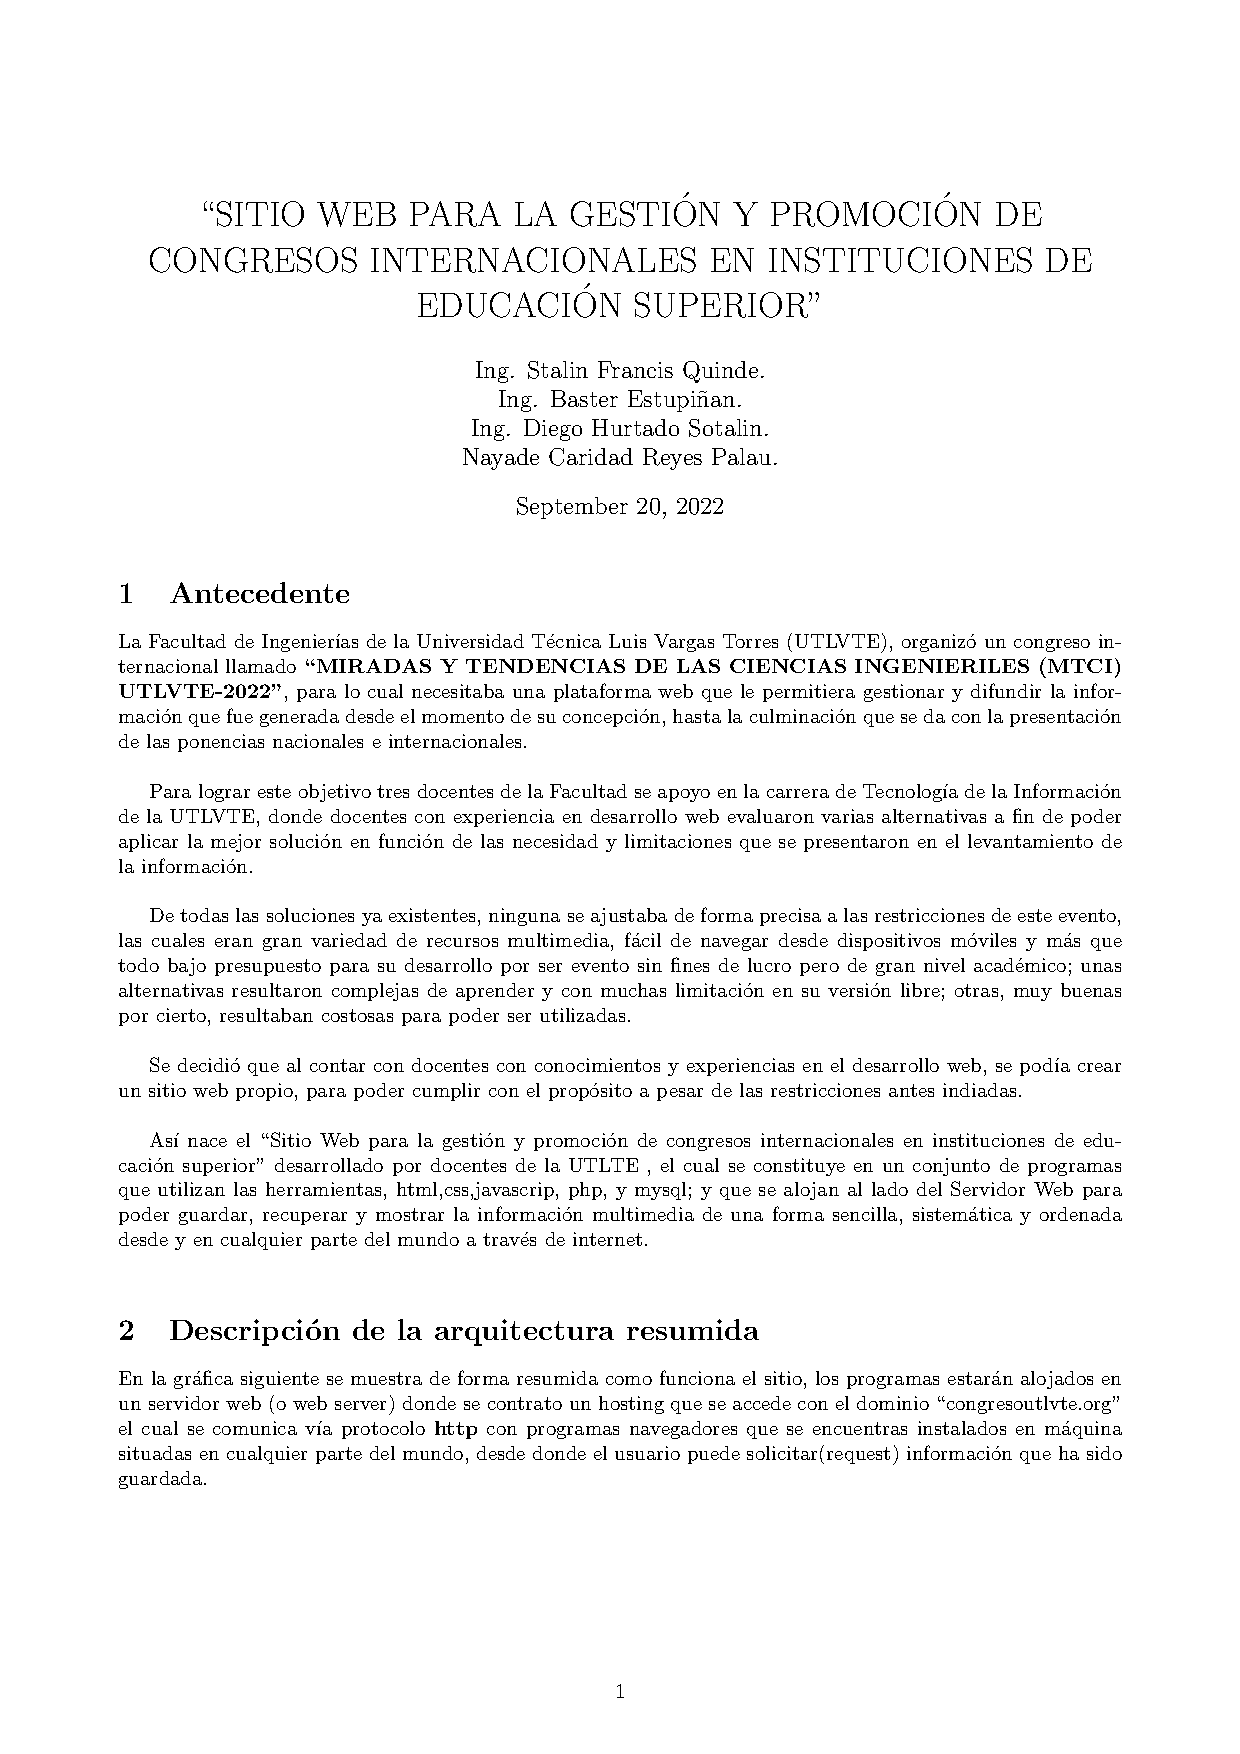
\includegraphics[scale=0.25]{congresoweb.jpg}
  \caption{Arquitectura y funcionamiento del Sitio Web}
  \label{fig:arquitectura}
\end{figure}


\subsection{El nombre del dominio}
\label{sec:nombres-del-dominio}

El sitio web esta alojado en un servidor al cual se puede acceder utilizando el nombre del dominio www.congresoutlvte.org; el nombre congresoutlvte se eligió considerando el tipo de evento(congreso) y el nombre de la institución (utlvte); la extensión (.org) se la escogió por el hecho de que los congresos realizados por la academia son eventos o actividades sin fines de lucro.


\subsection{Proveedor de servicios de Internet (PSI)}
\label{sec:prov-de-serv}

La empresa \textbf{REINEC}, fué la escogida para dar el servicio de alojamiento, la razón de su selección es por que cuenta con una buena reputación comporbada con más de 10 años trabajando con ella  y un servicio de soporte  técnico las 24 horas.

\subsection{Plan que se contrato.}
\label{sec:plan-que-se}

El plan que se contrató, es llamado \textbf{Hosting Junior PHP}; este plan permite crear un ilimitado número de correos utilizando el dominio @congresoutlvte.org, pero limita a solo crear 1 dominio adicional, la creación de tan solo hasta  3 base de datos y el almacenamiento de máximo 75000 archivos siempre y cuando no superen el tamaño de 15GB.  





\newpage
\section{Distribución de la información}



\subsection{Página principal}
\label{sec:pagina-principal}

En la figura 2 se muestra parte de la página principal del sitio web donde se pone a disposición información como logo de la universidad, banner promocional del congreso, resumen del congreso y fecha destacadas.

\begin{minipage}[H]{0.45\linewidth}
\begin{figure}[H]
  \centering
  \includegraphics[scale=0.3]{index1.jpg}
  \caption{index1.php }
  \label{fig:arquitectura1}
\end{figure}
  
\end{minipage}
\hspace{0.5cm}
        \begin{minipage}[H]{0.45\linewidth}
\begin{figure}[H]
  \centering
  \includegraphics[scale=0.3]{index2.jpg}
  \caption{index2.php }
  \label{fig:arquitectura2}
\end{figure}
  
\end{minipage}





\begin{minipage}[H]{0.45\linewidth}
\begin{figure}[H]
  \centering
  \includegraphics[scale=0.3]{index3.jpg}
  \caption{Se muestra conferencistas en primera página }
  \label{fig:arquitectura1}
\end{figure}
  
\end{minipage}
\hspace{0.5cm}
        \begin{minipage}[H]{0.45\linewidth}
\begin{figure}[H]
  \centering
  \includegraphics[scale=0.3]{index4.jpg}
  \caption{Se muestra los comites y sus miembros }
  \label{fig:arquitectura2}
\end{figure}
  
\end{minipage}













\newpage
\subsection{Página de presentación del congreso }
\label{sec:pagina-principal}

En la figura \ref{fig:presentacion}, se muestra el motivo, la visión, la misión y los  objetivos del congreso, información que forma parte de la presentación del evento.


\begin{figure}[H]
  \centering
  \includegraphics[scale=0.3]{presentacion.jpg}
  \caption{Presentación del congreso}
  \label{fig:presentacion}
\end{figure}

\newpage
\subsection{Página de normas de presentación }
\label{sec:pagina-principal}

Esta es la página  donde se muestra las normas a seguir para que los ponentes entreguen sus trabajos de forma correcta.


\begin{minipage}[H]{0.45\linewidth}
  \begin{figure}[H]
    \centering
    \includegraphics[scale=0.3]{normativas.jpg}
    \caption{Normativas}
    \label{fig:arquitectura}
  \end{figure}

\end{minipage}




\newpage
\subsection{Página de temáticas }
\label{sec:pagina-principal}

La conferencias preparadas por los ponentes debe realizarse en función de ejes temáticos definidos por la unidad de investigación de la Universidad auspiciante.

\begin{minipage}[H]{0.5\linewidth}
  \begin{figure}[H]
    \centering
    \includegraphics[scale=0.3]{tematicas.jpg}
    \caption{Temáticas}
    \label{fig:tematicas1}
  \end{figure}
\end{minipage}
\hspace{0.5cm}
\begin{minipage}[H]{0.5\linewidth}
  \begin{figure}[H]
    \centering
    \includegraphics[scale=0.3]{index2.jpg}
    \caption{Las temáticas tambien se muestran en la página principal}
    \label{fig:tematicas2}
  \end{figure}
\end{minipage}

\newpage
\subsection{Información de los  de confencistas }
\label{sec:pagina-principal}

La información de los conferencistas comienzan a mostrarse desde la primera página donde se presentan los conferencistas internacinales más destacados, los usuarios también tendrán acceso a una hoja de vida resumida para conocer detalles sobre el conferencista a más de un video de presentación.

  

\begin{minipage}[H]{0.5\linewidth}
  \begin{figure}[H]
    \centering
    \includegraphics[scale=0.3]{conferencistas.jpg}
    \caption{Lista de conferencxsistas}
    \label{fig:conferensistas}
  \end{figure}
\end{minipage}
\hspace{0.5cm}
\begin{minipage}[H]{0.5\linewidth}
  \begin{figure}[H]
    \centering
    \includegraphics[scale=0.3]{ponentes.jpg}
    \caption{Bibliografía del conferensista}
    \label{fig:bibliografia}
  \end{figure}
\end{minipage}




\begin{minipage}[H]{0.5\linewidth}
  \begin{figure}[H]
    \centering
    \includegraphics[scale=0.3]{bibliografia.jpg}
    \caption{Bibliografía resumida}
    \label{fig:conferensistas}
  \end{figure}
\end{minipage}
\hspace{0.5cm}
\begin{minipage}[H]{0.5\linewidth}
  \begin{figure}[H]
    \centering
    \includegraphics[scale=0.3]{bibliografia2.jpg}
    \caption{Bibliografía resumida}
    \label{fig:bibliografia}
  \end{figure}
\end{minipage}
  





\newpage
\subsection{Página para mostrar la memoria generada}
\label{sec:pagina-principal}

En esta página web se presenta todo los afíches generados y difundidos para dar a conocer el evento del congreso a realizarse..


\begin{figure}[H]
  \centering
  \includegraphics[scale=0.3]{memoria.jpg}
  \caption{Memoria}
  \label{fig:arquitectura}
\end{figure}

\newpage
\subsection{Página para inscripciones }
\label{sec:pagina-principal}

Esta página web permite acceder a un registro o formulario donde las personas que quieren participar en el congreso puedan dejar sus datos personales, datos que serán utilizados para generar los certificados respectivos.


\begin{minipage}[H]{0.45\linewidth}
  \begin{figure}[H]
    \centering
    \includegraphics[scale=0.3]{inscripcion.jpg}
    \caption{Inscripciones al congreso}
    \label{fig:arquitectura}
  \end{figure}
\end{minipage}
\begin{minipage}[H]{0.45\linewidth}
  \begin{figure}[H]
    \centering
    \includegraphics[scale=0.3]{inscripcion2.jpg}
    \caption{Formulario de inscripción}
    \label{fig:arquitectura2}
  \end{figure}
\end{minipage}


\newpage
\subsection{Información de los comites }

Los comites y sus integrantes que son los profesionales que trabajan antes, durante y después del evento, son mostrados en la primera página del sitio web. \\




\begin{minipage}[H]{0.45\linewidth}
  \begin{figure}[H]
    \centering
    \includegraphics[scale=0.3]{comite1.jpg}
    \caption{Sección donde se muestran los primeros 4 comites}
    \label{fig:comite1}
  \end{figure}
\end{minipage}
\begin{minipage}[H]{0.45\linewidth}
  \begin{figure}[H]
    \centering
    \includegraphics[scale=0.3]{comite2.jpg}
    \caption{Sección donde se muestran los últimos 4 comites}
    \label{fig:comite2}
  \end{figure}
\end{minipage}




\end{document}

%%% Local Variables:
%%% mode: latex
%%% TeX-master: t
%%% End:
